% ****** Start of file aipsamp.tex ******
%
%   This file is part of the AIP files in the AIP distribution for REVTeX 4.
%   Version 4.1 of REVTeX, October 2009
%
%   Copyright (c) 2009 American Institute of Physics.
%
%   See the AIP README file for restrictions and more information.
%
% TeX'ing this file requires that you have AMS-LaTeX 2.0 installed
% as well as the rest of the prerequisites for REVTeX 4.1
%
% It also requires running BibTeX. The commands are as follows:
%
%  1)  latex  aipsamp
%  2)  bibtex aipsamp
%  3)  latex  aipsamp
%  4)  latex  aipsamp
%
% Use this file as a source of example code for your aip document.
% Use the file aiptemplate.tex as a template for your document.
\documentclass[%
 aip,
 % apl,
% jmp,%
% bmf,%
% sd,%
% rsi,%
 amsmath,amssymb,
% preprint,%
 reprint,%
% author-year,%
% author-numerical,%
 floatfix,%
]{revtex4-1}

\usepackage[utf8]{inputenc}
\usepackage{tikz}
\usepackage{graphicx}% Include figure files
\usepackage{dcolumn}% Align table columns on decimal point
\usepackage[T1]{fontenc}
\usepackage{bm}% bold math
\usepackage{mathptmx}
%\usepackage[mathlines]{lineno}% Enable numbering of text and display math
%\linenumbers\relax % Commence numbering lines
\usetikzlibrary{arrows,decorations.markings,decorations.pathmorphing, patterns,shapes}

\begin{document}

\preprint{AIP/123-QED}

\title[]{The Double Pendulum:\\Creating a Better Baseball Bat}
%\thanks{Footnote to title of article.}

\author{Jared Baur}
%\altaffiliation[Also at ]{Physics Department, Occidental College.}%Lines break automatically or can be forced with \\

\date{\today}% It is always \today, today,
             %  but any date may be explicitly specified

\begin{abstract}
	abstract goes here
\end{abstract}

\maketitle

% \onecolumngrid

\section{\label{sec:level1}Introduction}

The double pendulum is a classic example of chaotic motion\cite{Shinbrot1992}. The trajectories of various trials will show that the motion of a double pendulum is highly unpredictable. The chaos in a classic double pendulum is described by Equation 1. The exponent $\lambda$ is a positive constant, $\Delta x$ is the trajectory of the bottom arm of the pendulum, and $t$ is time. For small times $t$, the trajectories are relatively the same, however for increasing times, the trajectories exponentially increase in distance from trial to trial.
\begin{equation}
	\Delta x(t) \sim \Delta x(t_0) e^{\lambda t}
\end{equation}

\begin{figure}
	\centering
	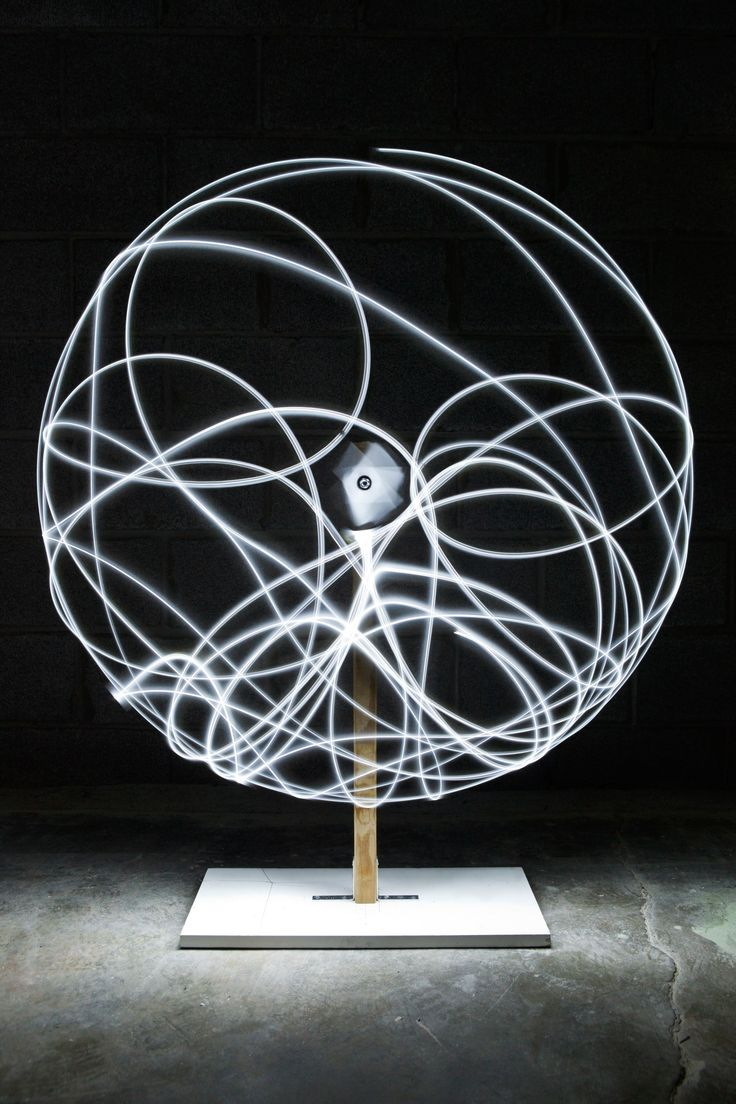
\includegraphics[scale=0.25]{lights.jpg}
	\caption{Chaos in a double pendulum. This figure depicts the trajectory of the end of the bottom arm in the double pendulum. The light is traced along the route of the bottom arm. As seen, there is no evident pattern in the bottom arm's trajectory.}
\end{figure}

The double pendulum is used in real life situations such as in double-trailer trucks (officially known as ``long combination vehicles") where two large-wheeled vehicles are combined at a hinge point. These vehicles are essentially semi-trucks with two trailers attached instead of one. The swinging motion in sports is also a common instance of a double pendulum. For this paper, the double pendulum will be compared to a baseball swing. In a baseball swing, a bat (striking implement) is used in conjunction with the arms to strike a baseball. In general, the arms are held up and back from the player's head, with the bat pointed upwards. The arms initiate the swing, moving towards the center of the player's body; the bat follows the arms, and then swings through as the transfer of energy from the arms to the bat occurs. This motion occurs mostly in the horizontal plane, but nonetheless acts as a double pendulum with the player's arms and the bat as the upper and lower ``arms" of the pendulum, respectively.

Since the swing of a baseball bat only occurs once per trial (does not swing back and forth and time $t$ is relatively low), this motion is equivalent to the first half cycle of a double pendulum swing. Thus, the chaotic motion prevalent in classic double pendulums will not be applicable for the purpose of the baseball swing.

Although the focus of this paper will be on the baseball swing, the double pendulum motion can be applied to the motion of a swing of a baseball bat, golf club, tennis racquet, or any other "swinging" motion that occurs with a striking implement. The goal of this paper will be to quantitatively describe the double pendulum in the context of a baseball swing and determine whether all of the energy in the striking implement can be transferred to the ball on impact. From this, we will decide whether we can design a baseball bat or ball that would allow for this perfect transfer of energy to occur.

\section{\label{sec:level2}Equations of Motion}

Describing the motion of a double pendulum has been argued as highly complicated\cite{Jorgensen1970}. For this reason, Lagrangians have been used in past studies to represent this motion. However, when we look at the forces on each arm of the pendulum with respect to each arm's center of mass, Newtonian equations of motion can be used to describe the motion.

Figure 2 depicts the components in a simple double pendulum. The $x,y$ axes for position and forces are shown in the figure. The upper arm of the pendulum is the first arm attached to a fixed axis $A$. This arm has length $L_1$, center of mass at point $G_1$, and distance to its center of mass $h_1$ (measured from point $A$). This arm makes an angle $\theta$ with the vertical axis and has a gravitational force acting on its center of mass equal to $M_1 g$, where $M_1$ is the mass of the arm and $g$ is the acceleration due to gravity.

The second arm (lower arm) rotates on a ``fixed" axis at point $B$. If we isolate the second arm from the system, it would rotate about point $B$ as if it were fixed, however point $B$ is rotating around point $A$ since it is at the end of the first arm. The second arm has a length $L_2$ and its center of mass at point $G_2$, a distance of $h_2$ away from point $B$. The arm makes an angle of $\phi$ with the vertical axis and has a gravitational force of $M_2 g$ acting on its mass $M_2$. Point C is the end of the second arm, and will act as a point of interest for our paper as we track the trajectory of this point. The velocity vector $V$ is the direction of motion for the second arm's center of mass through the swinging of a double pendulum. 
\begin{figure}
	\centering
	\begin{tikzpicture}
		\node [inner sep=0pt,above right]
		{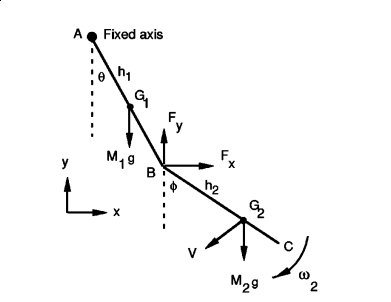
\includegraphics[scale=0.6]{equationsofmotion.png}};

		\draw[<->] (2,2.85) -- (0.5,5.5);
		\node (none) at (1,3.8) {$L_1$};

		\draw[<->] (5.5,2.85) -- (7.9,1.3);
		\node (none) at (6.9,2.4) {$L_2$};

	\end{tikzpicture}
	\caption{The components in a double pendulum. Since the equations that describe a double pendulum can be rather confusing, we use the center of mass $G_1$ and $G_2$ to describe the forces acting on the pendula arms.}
\end{figure}

We start writing our equations of motion by describing the coordinates of our center of mass on the second arm. We want the coordinates of the center of mass since we will write our forces with respect to that (as opposed to point C). Point $G_2$ is described in Equation 2, where the first half of the equation is the $x$ component and the second half is the $y$ component. The $y$ component is negative since the double pendulum's origin at $(x,y)=(0,0)$ is assumed at point $A$.

\begin{equation}
	G_2(x,y) = \Big([L_1 \sin{\theta} + h_2 \sin{\phi}],  [- L_1 \cos{\theta} - h_2 \cos{\phi}]\Big)
\end{equation}

The velocity of point $G_2$ is found by using the angular velocity of the entire first arm, $\omega_1$, and combining it with the angular velocity of the second arm, $\omega_2$. The components of this velocity are found by multiplying the angular velocities against the distance to point $G_2$. For the $x$-direction, we take $-L_1 \cos{\theta}$ for the first arm and $-h_2 \cos{\phi}$ for the second arm. Likewise for the $y$-direction, we take $-L_1 \sin{\theta}$ and $-h_2 \sin{\phi}$ for the first and second arms, respectively. These components are oriented negatively since the arm is moving in the negative $x$- and $y$-directions. The velocities $V_x$ and $V_y$ for point $G_2$ are described in Equations 3 and 4.

\begin{equation}
	V_x = \frac{dx}{dt} = -L_1 \omega_1 \cos{\theta} - h_2 \omega_2 \cos{\phi}
\end{equation}

\begin{equation}
	V_y = \frac{dy}{dt} = -L_1 \omega_1 \sin{\theta} - h_2 \omega_2 \sin{\phi}
\end{equation}

The forces on center of mass point $G_2$ are found by taking the derivatives of Equations 3 and 4. Newton's second law $\sum \bold{F} = m \bold{a}$ is used to describe the sum of forces acting on the double pendulum. For the force in the $x$-direction, the only force applied to $G_2$ is the force from the upper arm pulling on the lower arm. For the $y$-direction, the upper arm as well as force due to gravity act on the lower arm. The $x$- and $y$-components of force are given by Equations 5 and 6.

\begin{equation}
	\begin{aligned}
		F_x & = M_2 \frac{d V_x}{dt} \\
		    & = -M_2 \bigg [ L_1 \cos{\theta} \frac{d \omega_1}{dt} + L_1 \omega_1^2 \sin{\theta} \\
		    & + h_2 \cos{\phi} \frac{d \omega_2}{dt} + h_2 \omega_2^2 \sin{\phi} \bigg ]
	\end{aligned}
\end{equation}

\begin{equation}
	\begin{aligned}
		F_y - M_2 g & = M_2 \frac{d V_y}{dt}\\
		   & = -M_2 \bigg [ L_1 \sin{\theta} \frac{d \omega_1}{dt} - L_1 \omega_1^2 \cos{\theta} \\
		   & + h_2 \sin{\phi} \frac{d \omega_2}{dt} - h_2 \omega_2^2 \cos{\phi} \bigg ]
	\end{aligned}
\end{equation}

These derived equations are for a generic double pendulum that falls in a vertical fashion. In order to apply this concept to the swing of a baseball bat, we will use the torques on the pendula components. The terminology we will use for the upper and lower components of the pendulum will be the ``arm" and ``rod", respectively. In a baseball swing, the upper body musculature applies

\section{\label{sec:level3}Experimental Results}

\section{\label{sec:level4}Torque}

\section{\label{sec:level5}Energy Transfer}

\section{\label{sec:level6}Conclusion}

\nocite{*}
\bibliography{main.bib}% Produces the bibliography via BibTeX.

\end{document}
%
% ****** End of file aipsamp.tex ******
